\documentclass[tikz]{standalone}

\usetikzlibrary{patterns}

\begin{document}

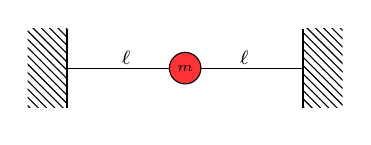
\begin{tikzpicture}
    \fill[pattern=north west lines] (0,0) rectangle ++(0.5,1);
    \draw[thick] (0.5,0)--(0.5,1);
    \fill[pattern=north west lines] (3.5,0) rectangle ++(0.5,1);
    \draw[thick] (3.5,0)--(3.5,1);
    \draw (0.5,0.5)--(3.5,0.5);
    \filldraw[color=black, fill=red!80](2,0.5) circle (0.2) node {\tiny{$m$}};
    \node[label={[shift={(0,0.3)}]$\scriptstyle{\ell}$}] at (1.25,0){};
    \node[label={[shift={(0,0.3)}]$\scriptstyle{\ell}$}] at (1.25+1.5,0){};
\end{tikzpicture}

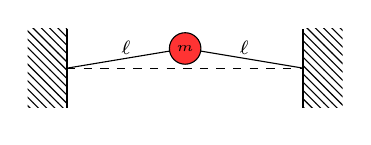
\begin{tikzpicture}
    \fill[pattern=north west lines] (0,0) rectangle ++(0.5,1);
    \draw[thick] (0.5,0)--(0.5,1);
    \fill[pattern=north west lines] (3.5,0) rectangle ++(0.5,1);
    \draw[thick] (3.5,0)--(3.5,1);
    \draw (0.5,0.5)--(2,0.75);
    \draw (2,0.75)--(3.5,0.5);
    \filldraw[color=black, fill=red!80](2,0.75) circle (0.2) node {\tiny{$m$}};
    \node[label={[shift={(0,0.42)}]$\scriptstyle{\ell}$}] at (1.25,0){};
    \node[label={[shift={(0,0.42)}]$\scriptstyle{\ell}$}] at (1.25+1.5,0){};
    \draw[dashed] (0.5,0.5)--(3.5,0.5);
\end{tikzpicture}

\end{document}